% Options for packages loaded elsewhere
% \PassOptionsToPackage{unicode}{hyperref}
% \PassOptionsToPackage{hyphens}{url}
%
\documentclass[
  12pt,
  answers  
]{exam}
\usepackage[fleqn]{amsmath}
\usepackage[]{plex-otf}
\usepackage{iftex}
\usepackage[a4paper, margin=2.5cm]{geometry}

% \ifPDFTeX
%   \usepackage[T1]{fontenc}
%   \usepackage[utf8]{inputenc}
%   \usepackage{textcomp} % provide euro and other symbols
% \else % if luatex or xetex
%   \usepackage{unicode-math}
%   \defaultfontfeatures{Scale=MatchLowercase}
%   \defaultfontfeatures[\rmfamily]{Ligatures=TeX,Scale=1}
% \fi
% Use upquote if available, for straight quotes in verbatim environments
\IfFileExists{upquote.sty}{\usepackage{upquote}}{}
\IfFileExists{microtype.sty}{% use microtype if available
  \usepackage[]{microtype}
  \UseMicrotypeSet[protrusion]{basicmath} % disable protrusion for tt fonts
}{}
\makeatletter
\makeatother
\usepackage{xcolor}
\IfFileExists{xurl.sty}{\usepackage{xurl}}{} % add URL line breaks if available
\IfFileExists{bookmark.sty}{\usepackage{bookmark}}{\usepackage{hyperref}}
\urlstyle{same} % disable monospaced font for URLs
\setlength{\emergencystretch}{3em} % prevent overfull lines
\providecommand{\tightlist}{%
  \setlength{\itemsep}{0pt}\setlength{\parskip}{0pt}}
\setcounter{secnumdepth}{-\maxdimen} % remove section numbering
\newlength{\cslhangindent}
\setlength{\cslhangindent}{1.5em}
\newlength{\csllabelwidth}
\setlength{\csllabelwidth}{3em}
\newlength{\cslentryspacingunit} % times entry-spacing
\setlength{\cslentryspacingunit}{\parskip}
\newenvironment{CSLReferences}[2] % #1 hanging-ident, #2 entry spacing
 {% don't indent paragraphs
  \setlength{\parindent}{0pt}
  % turn on hanging indent if param 1 is 1
  \ifodd #1
  \let\oldpar\par
  \def\par{\hangindent=\cslhangindent\oldpar}
  \fi
  % set entry spacing
  \setlength{\parskip}{#2\cslentryspacingunit}
 }%
 {}
\usepackage{calc}
\newcommand{\CSLBlock}[1]{#1\hfill\break}
\newcommand{\CSLLeftMargin}[1]{\parbox[t]{\csllabelwidth}{#1}}
\newcommand{\CSLRightInline}[1]{\parbox[t]{\linewidth - \csllabelwidth}{#1}\break}
\newcommand{\CSLIndent}[1]{\hspace{\cslhangindent}#1}
\ifLuaTeX
  \usepackage{selnolig}  % disable illegal ligatures
\fi

\newcommand{\mytitle}{}
\newcommand{\theauthor}{Rivo Juicer Wowor}
\newcommand{\affiliation}{00000059635}

% \title{\textbf{\mytitle}}
% \author{\theauthor \
		% \small{\affiliation}}
% \date{}

% \usepackage{fancyhdr}
% \fancypagestyle{plain}{%
%   \fancyhf{}%
%   \lhead{\footnotesize{\textbf{\mytitle}}}%
%   % \rhead{\small{\textbf{Rivo Juicer Wowor (00000059635)}}}%
%   \fancyfoot[R]{\thepage}%
%   \fancyfoot[L]{\footnotesize{\theauthor \hspace{1pt} (\affiliation)}}
%   \renewcommand{\headrulewidth}{0.4pt}% Line at the header invisible
%   \renewcommand{\footrulewidth}{0.4pt}% Footer line not visible with 0pt
% }
\usepackage{graphicx}
\pagestyle{plain}
\setlength{\parindent}{2em}
\renewcommand{\baselinestretch}{1.5}
\usepackage{listings}
\lstdefinestyle{mystyle}{
	showtabs=false,                  
    tabsize=3,
	basicstyle=\linespread{0.6}
}
\lstset{style=mystyle}
\usepackage{booktabs, multirow}

\begin{document}
	\section{Pertanyaan Teori}
	\begin{questions}
		\question Apa perbedaan antara algoritma dan program?
	\begin{solution}
		Algoritma berfungsi untuk memberikan solusi masalah dalam bentuk Langkah-langkah. Sedangkan program berfungsi untuk menjalankan dari solusi algoritma.
	\end{solution}

	\question Apakah yang dimaksud dengan algoritma?
	\begin{solution}
		Algoritma merupakan deskripsi yang menjelaskan apa yang harus dikerjakan. Algoritma bisa disebut juga yaitu resep, langkahnya seperti \emph{"Panggang sampai selesai"} tidak jelas karena tidak menjelaskan apa yang berarti \emph{"selesai"}.
	\end{solution}

		\question Apa yang dimaksud dengan flowchart dan pseudocode?
	\begin{solution}
		Flowchart adalah sebuah cara merepresentasikan algoritma dengan menggunakan simbol-simbol geometris dan grafik. Sedangkan Pseudocode adalah sebuah cara merepresentasikan algoritma dengan menggunakan bahasa sehari-hari
	\end{solution}

		\question Sebutkan fungsi desk checking? 
	\begin{solution}
		Desk checking adalah suatu teknik manual yang digunakan untuk memeriksa logika dari suatu algoritma. Manfaatnya untuk melakukan proses pengecekan algoritma sebelum membuat program untuk mengurangi kesalahan.
	\end{solution}
	
		\question Suatu algoritma terdiri dari tiga struktur dasar, yaitu runtunan, pemilihan, dan perulangan. Jelaskan masing-masing!
	\begin{solution}
		\begin{enumerate}
			\item Algoritma runtunan merupakan sekumpulan perintah atau pernyataan yang dikerjakan komputer berdasarkan dengan urutan perintahnya.
			\item Algoritma perulangan adalah proses yang digunakan untuk mengulang beberapa perintah sesuai dengan jumlah yang telah ditentukan.
			\item Algoritma pemilihan adalah proses yang dilakukan sesuai dengan persyaratan atau kondisi tertentu yang sudah terpenuhi.
		\end{enumerate}
	\end{solution}
	\question Kapan modularisasi dibutuhkan dalam pembuatan algoritma?
	\begin{solution}
		Ketika source code program sudah terlalu besar dan kompleks, maka dapat dipecahkan menjadi beberapa modul. Fungsi modul supaya kita membacanya lebih tertata. Dengan begitu, bisa diimplementasikan jauh lebih mudah dipahami.
	\end{solution}
	\question Sebutkan kelebihan dan kekurangan menggunakan modularisasi dalam pembuatan algoritma? 
	\begin{solution}
		\newline
		Kelebihan: kodenya bisa dipakai kembali, mengurangi pengulangan penulisan, memudahkan dipahami, dan proses maintenance yang lebih efisien. 

		Kekurangan: jika dibagi terlalu banyak dan kecil akan kurang efisien
	\end{solution}
	\end{questions}
	\pagebreak

	\section{Lengkapi penulisan flowchart berikut ini}
	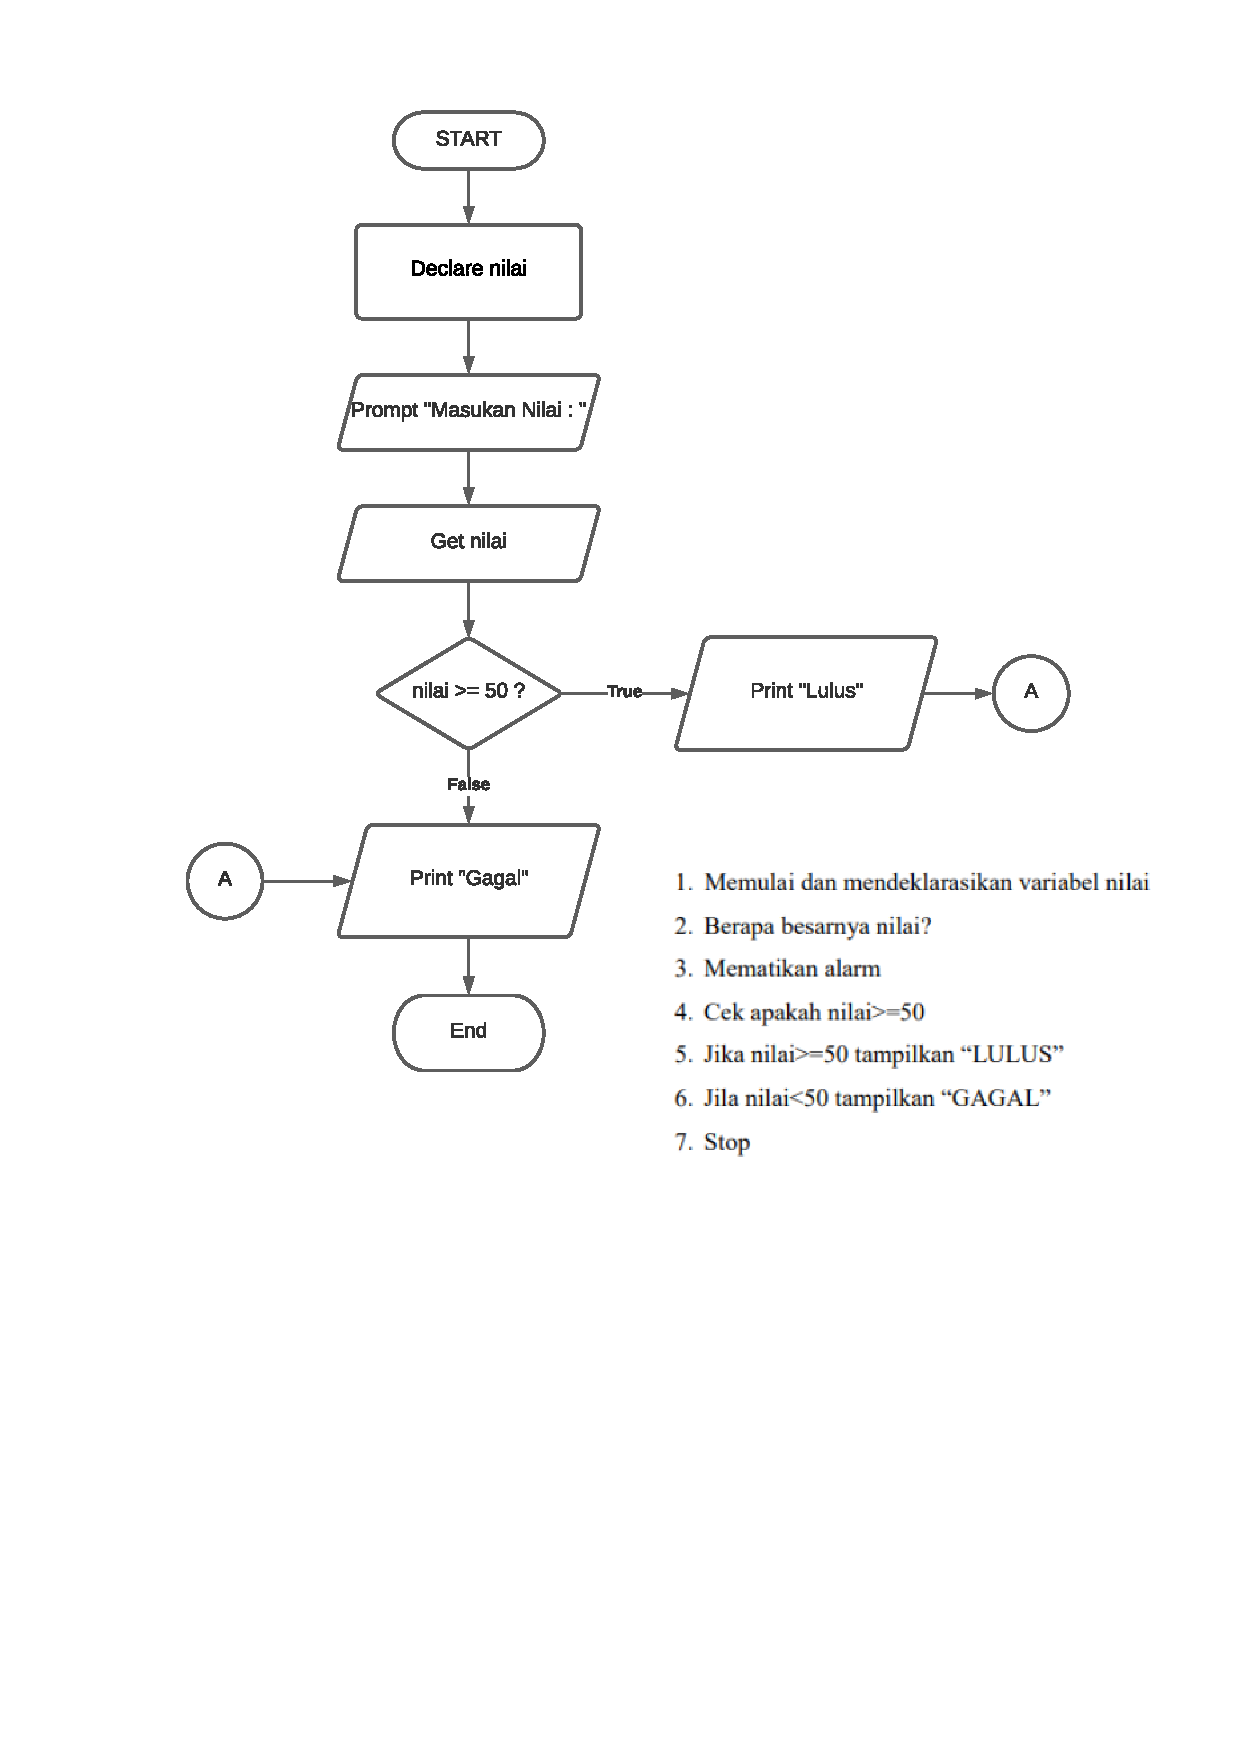
\includegraphics[clip, scale=0.9, trim={3cm 0 0 0}]{pdf/ProfunKelompok-1.pdf}

	\section{Analisalah flowchart dibawah ini dan selanjutnya lengkapilah trace table!} 
	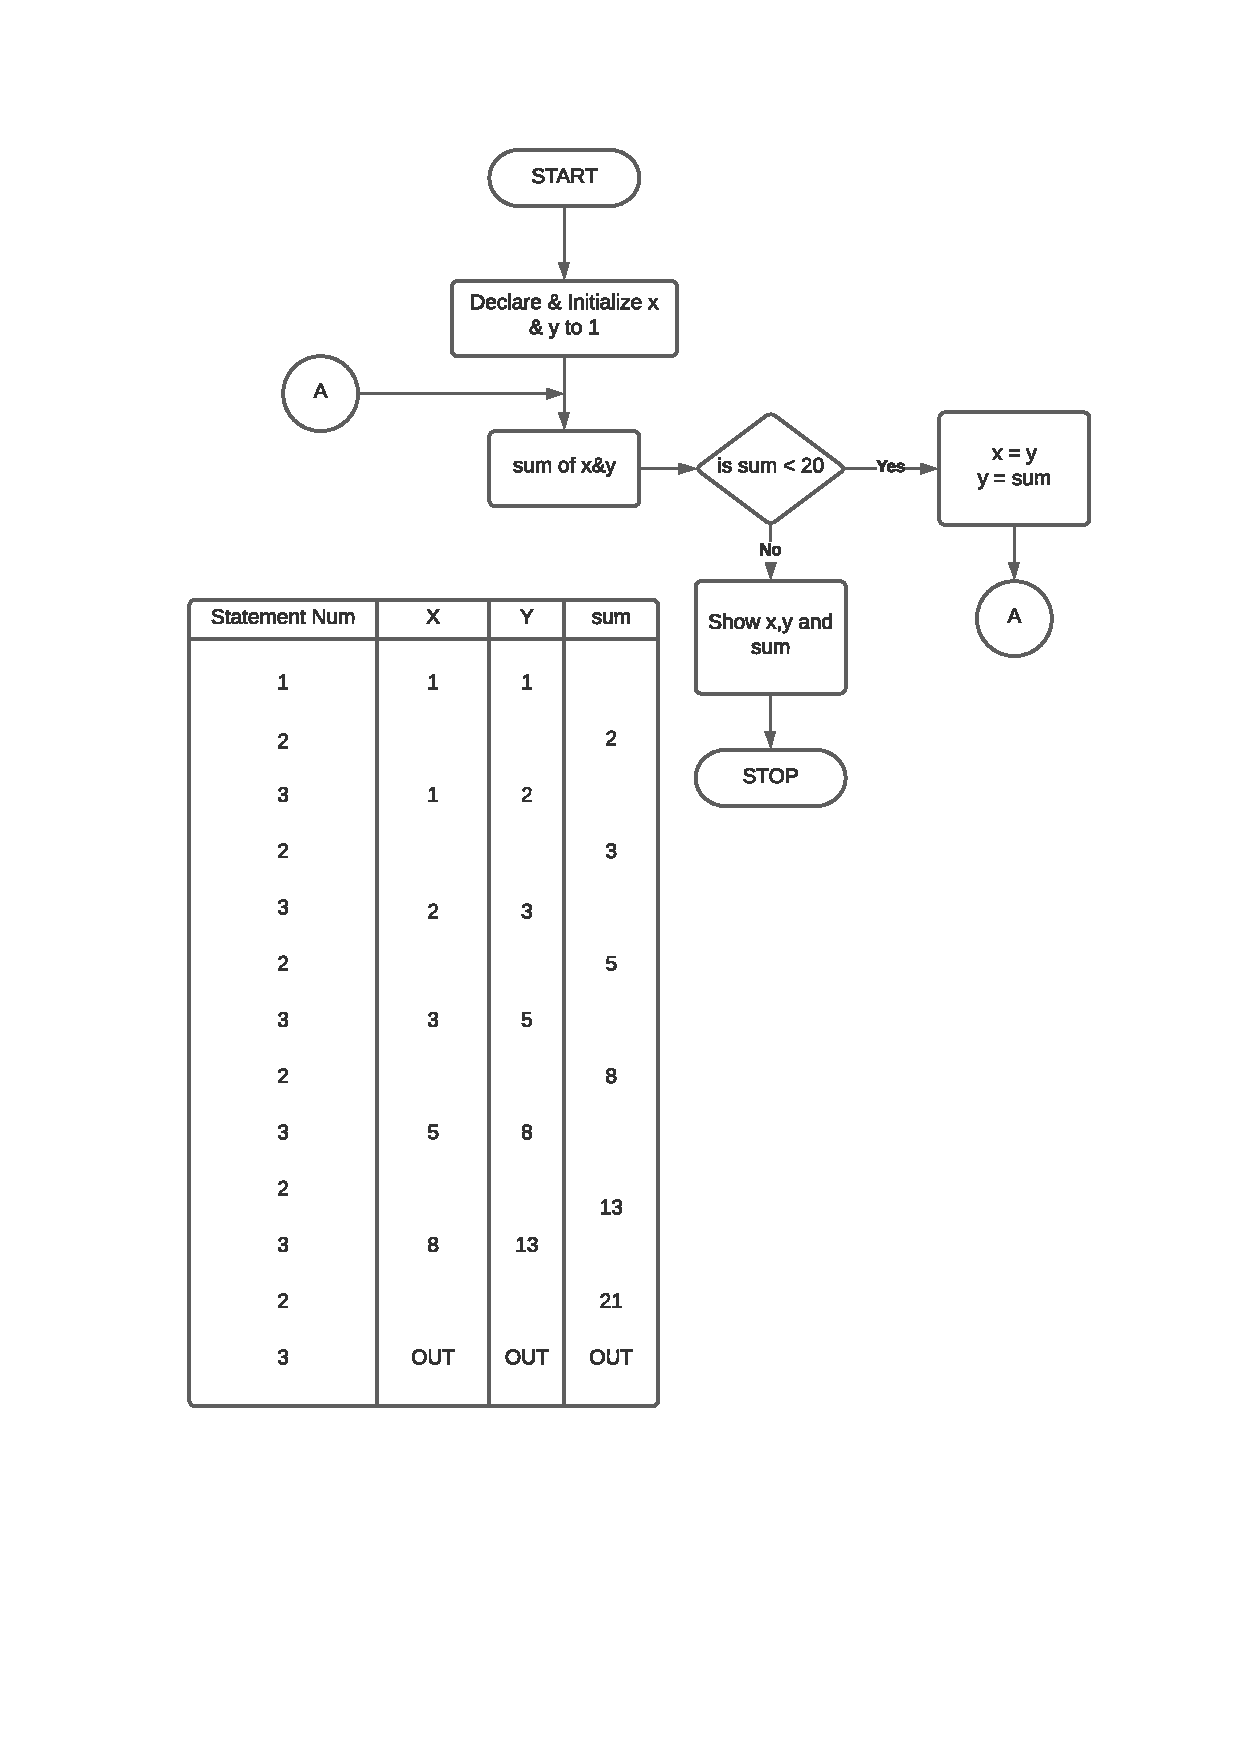
\includegraphics[clip, scale=0.9,trim={2cm 1cm 0 2cm}]{pdf/ProfunKelompok-2.pdf}

	\section{Flowchart dan Pseudocode}
	\subsection*{Problem 1}
	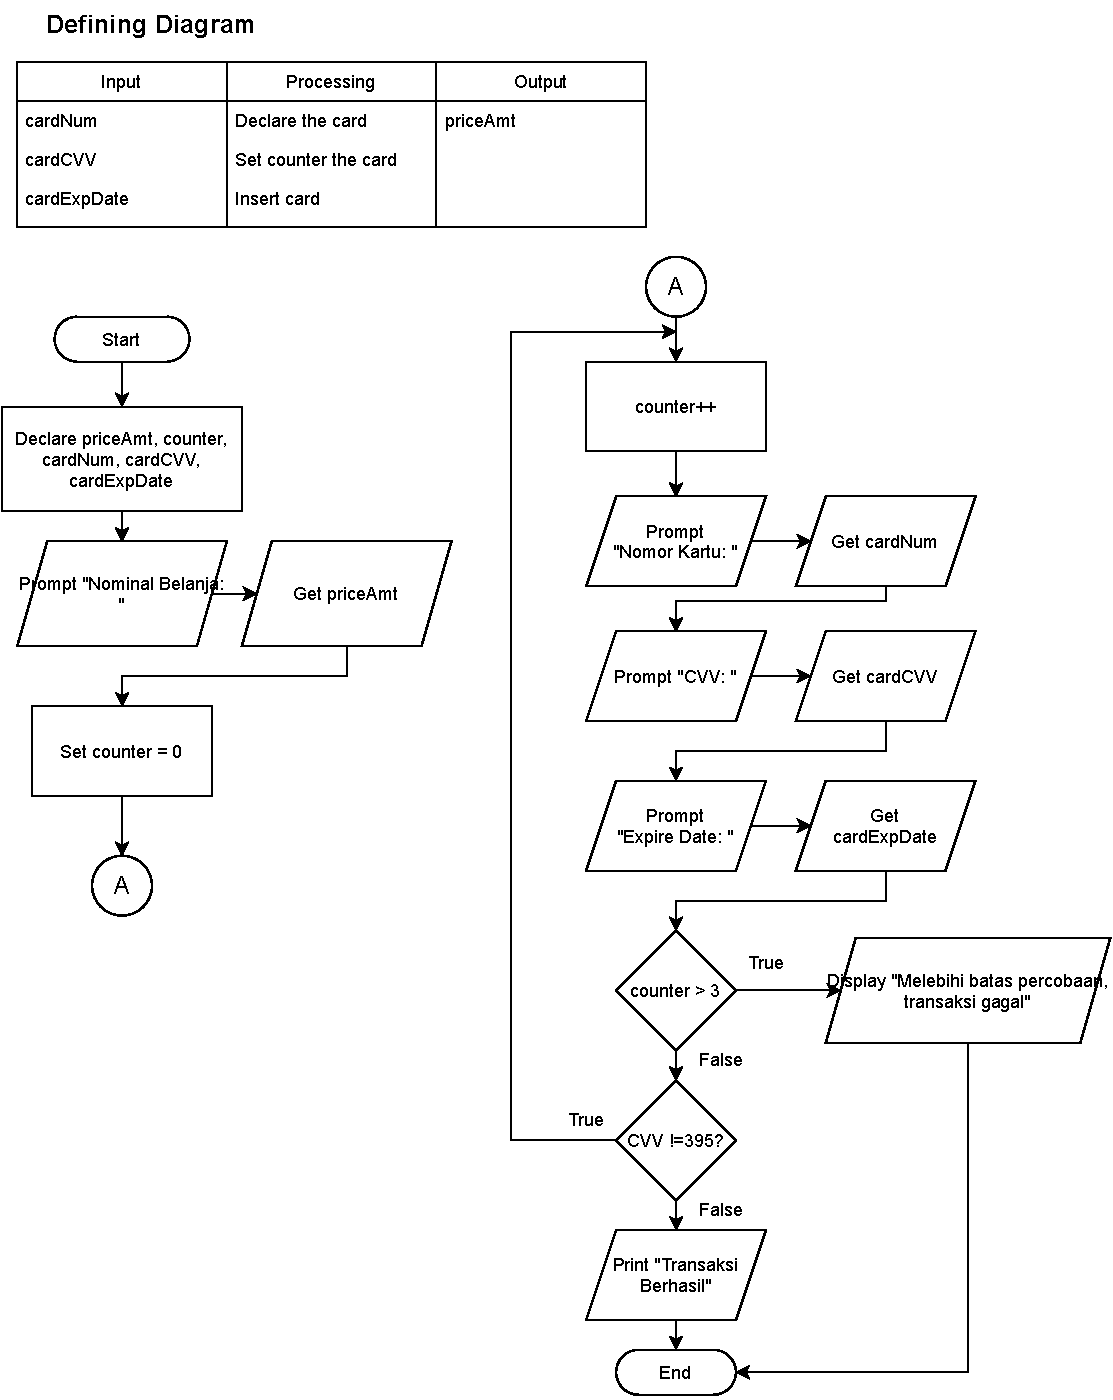
\includegraphics[clip, scale=0.8]{pdf/1-Problem1.pdf}
	\pagebreak
	\subsubsection*{Pseudocode}
	\begin{lstlisting}
1	Deklarasikan priceAmt, counter, cardNum, 
	cardCVV, dan cardExpDate
2	Masukkan nominal belanja dan isi di variabel priceAmt
	Lakukan:
3		Tambahkan 1 kedalam counter
4		Masukkan nomor kartu dan isi di variabel cardNum
5		Masukkan CVV dan isi di variabel cardCVV
6		Masukkan Expiration Date dan isi di variabel cardExpDate
7		Jika counter > 3, maka:
 			Berikan error
 			Hentikan program
 	Selama CVV != 395
8	Print "Transaksi Berhasil!"
	\end{lstlisting}
	\subsubsection*{Desk Checking}
	\begin{center}
		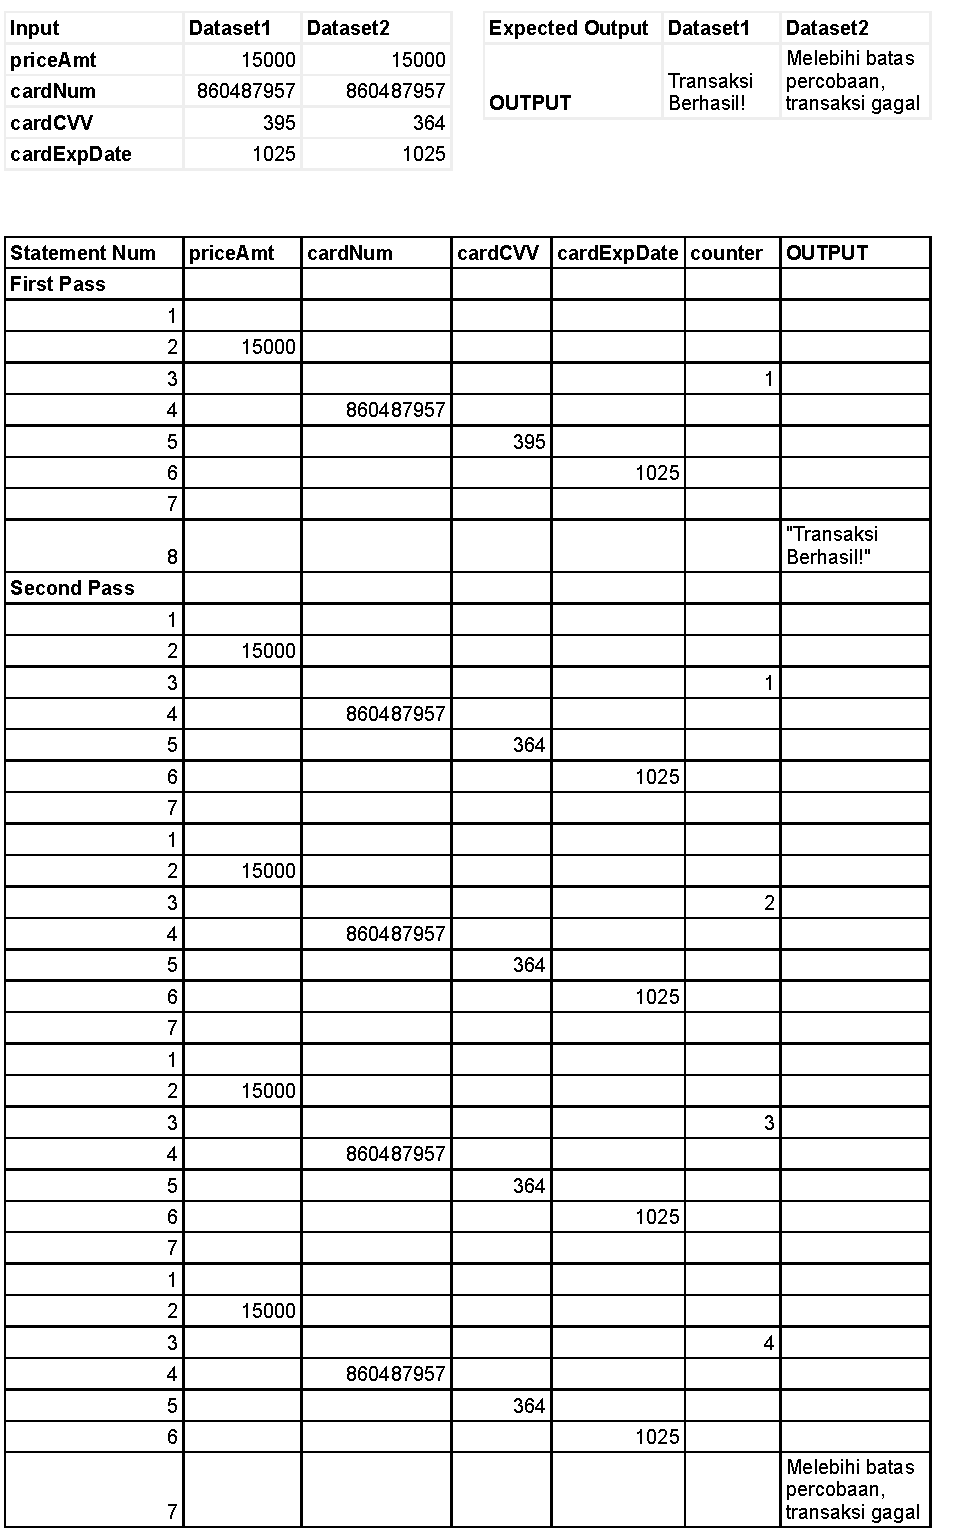
\includegraphics[clip, scale=0.92]{pdf/1-Problem1DC.pdf}
	\end{center}

	\pagebreak

	\subsection*{Problem 2}
	\begin{center}
		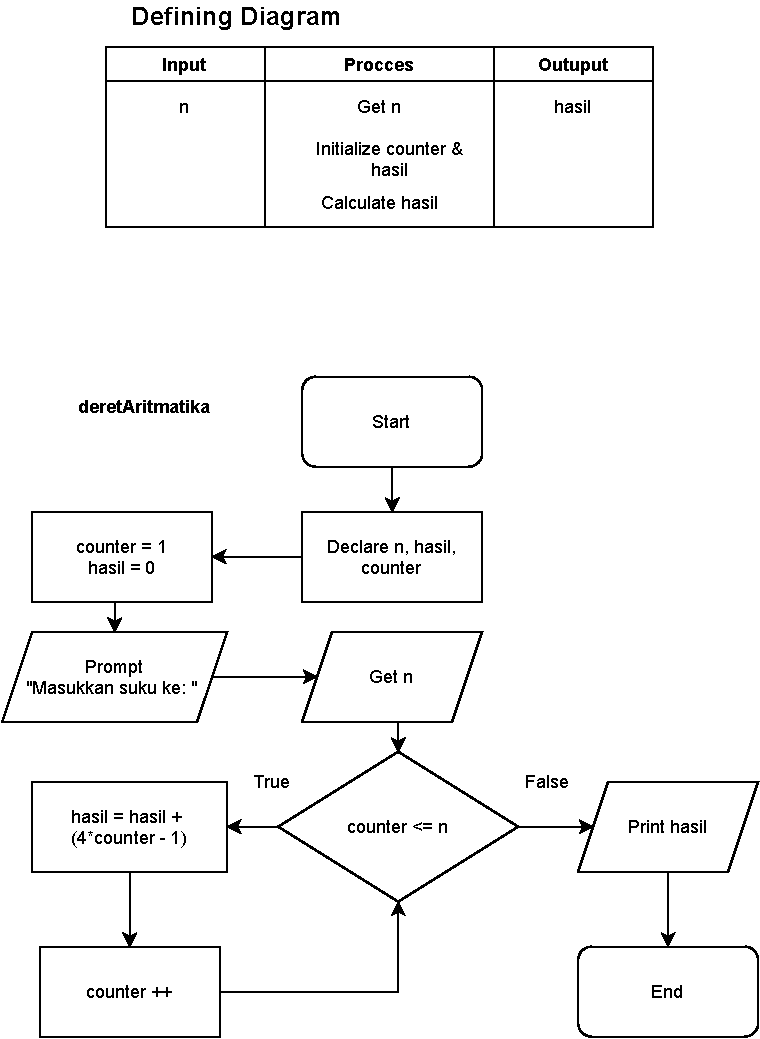
\includegraphics{pdf/Problem2.pdf}
	\end{center}

	\pagebreak
	\subsubsection*{Pseudocode}
	\begin{lstlisting}
1	Deklarasikan variabel n, counter dan hasil
2	Isi variabel hasil dengan angka 0
	Isi variabel counter dengan angka 1
3	Masukkan nilai suku dan isi di variabel n
	Selama counter kurang dari atau sama dengan n:
4		Isi variabel hasil dengan isi dari variabel hasil
		ditambah hasil dari rumus (4*counter-1)
5		Tambahkan satu pada counter
6	Munculkan isi dari variabel hasil
	\end{lstlisting}
	\pagebreak
	\subsubsection*{Desk Checking}
	\begin{center}
		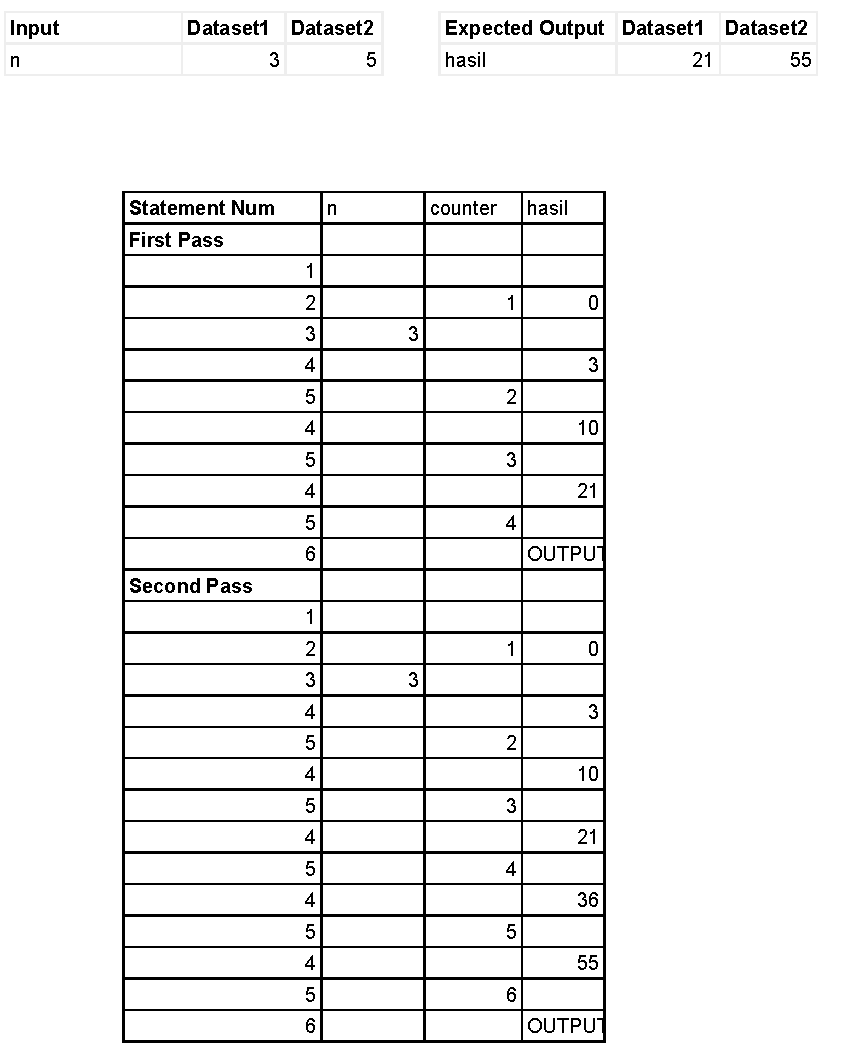
\includegraphics{pdf/Problem2DC.pdf}
	\end{center}

	\subsection*{Problem 3}
	\begin{center}
		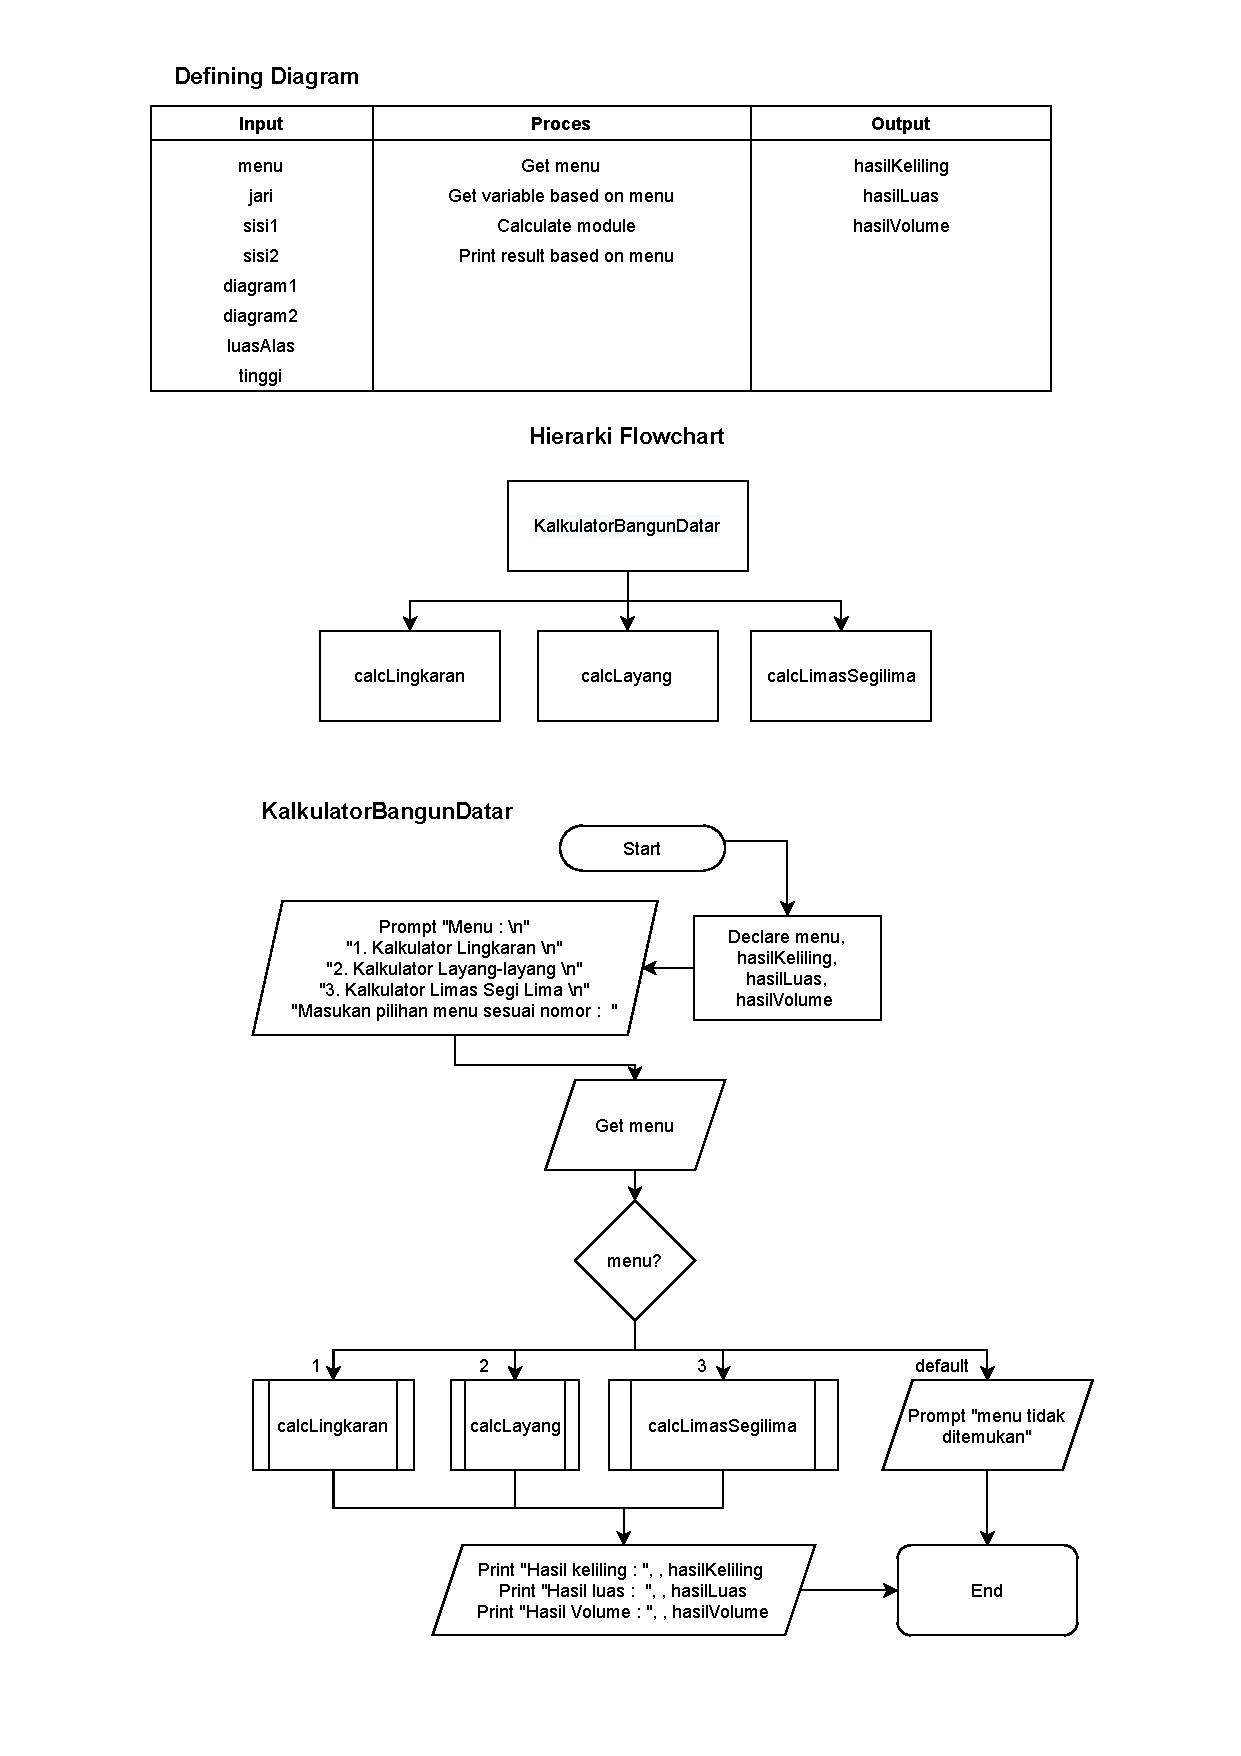
\includegraphics[clip, scale=0.85, trim={2cm 0.5cm 2cm 0.5cm}]{pdf/Problem3-1.pdf}
	\end{center}
	\pagebreak
	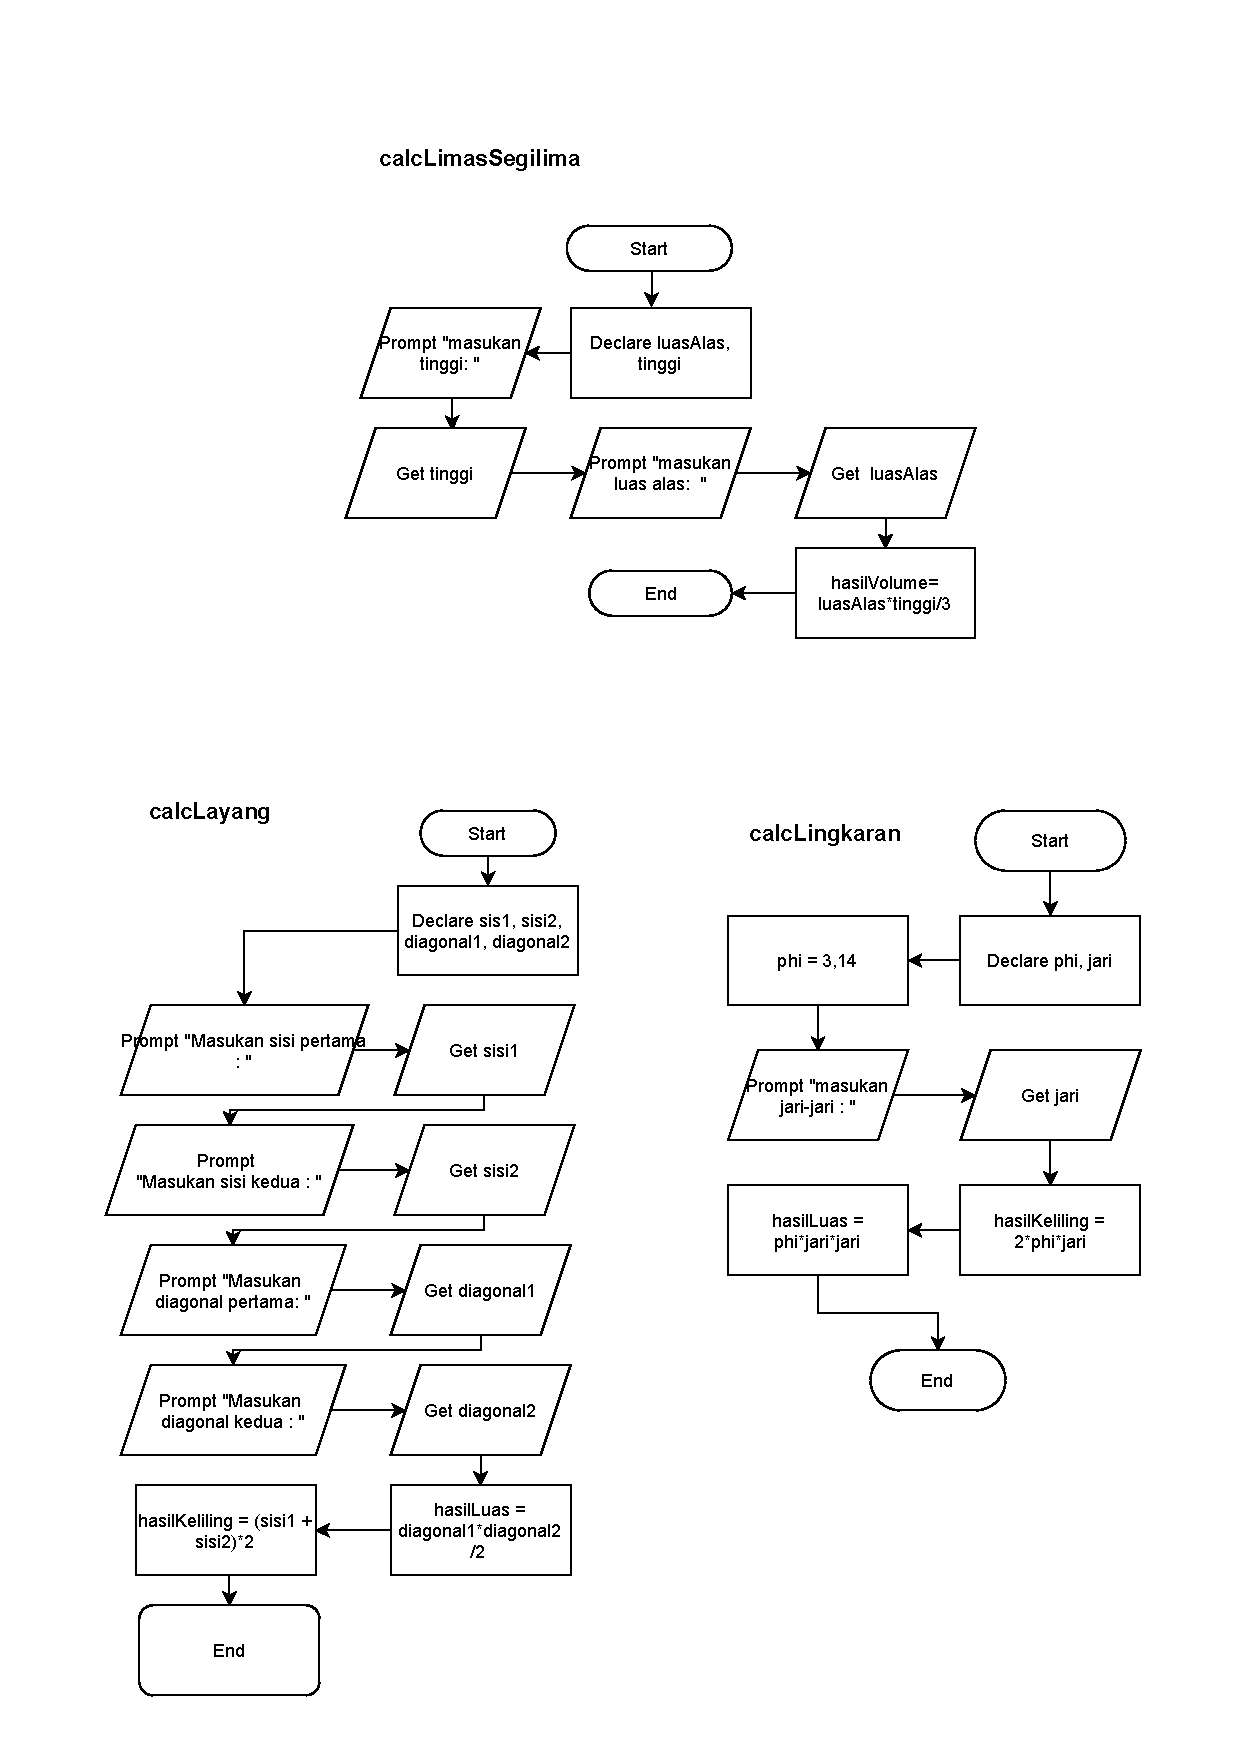
\includegraphics[clip, scale=0.85, trim={2cm 0.5cm 1cm 0.5cm}]{pdf/Problem3-2.pdf}

	\subsubsection*{Pseudocode}
	\begin{lstlisting}
kalkulatorBangunDatar
START
1	DECLARE menu, hasilKeliling, hasilLuas, hasilVolume
2	PRINT "1. Kalkulator Lingkaran"
	PRINT "2. Kalkulator Layang-layang"
	PRINT "3. Kalkulator Limas Segilima"
3	PROMPT "Pilih menu: "
	GET menu
		
4	CASE of menu
		1: calcLingkaran
		2: calcLayang
		3: calcLimasSegilima
		default: PRINT "Menu tidak ditemukan"
	ENDCASE

5	PRINT "Hasil Keliling: ", hasilKeliling
	PRINT "Hasil Luas: ", hasilLuas
	PRINT "Hasil Volume: ", hasilVolume
END
	
calcLingkaran
START
1	DECLARE phi, jari
2	phi = 3.14
3	PROMPT "Masukkan jari-jari: "
	GET jari

4	hasilKeliling = 2 * phi * jari
5	hasilLuas = phi * jari * jari
END

calcLayang
START
1	DECLARE sisi1, sisi2, diagon1, diagon2
2	PROMPT "Masukkan panjang sisi pertama: " 
	GET sisi1
	PROMPT "Masukkan panjang sisi kedua: " 
	GET sisi2
	PROMPT "Masukkan panjang diagonal pertama: " 
	GET diagon1 
	PROMPT "Masukkan panjang diagonal kedua: " 
	GET diagon2 
	
3	hasilKeliling = 2 * (sisi1 + sisi2)
4	hasilLuas = (diagon1 + diagon2) / 2
END

calcLimasSegilima
START
1	DECLARE luasAlas, tinggi
2	PROMPT "Masukkan luas alasnya: " 
	GET luasAlas
	PROMPT "Masukkan tinggi: " 
	GET tinggi

3	hasilVolume = (luasAlas * tinggi) / 3
END
	\end{lstlisting}
	\subsubsection*{Desk Checking}
	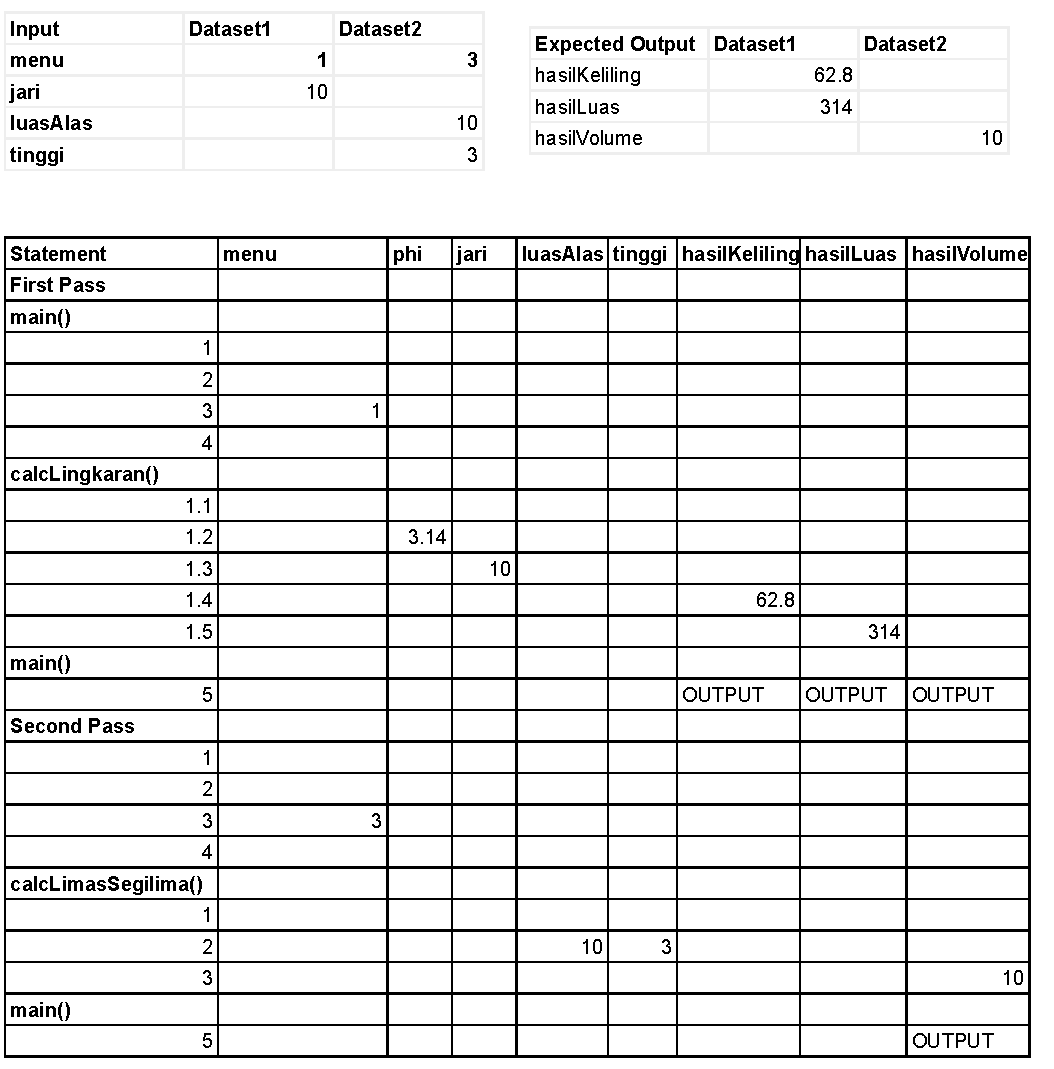
\includegraphics[clip, scale=0.93]{pdf/Problem3DC.pdf}
	\pagebreak

	\subsection*{Problem 4}
	\begin{center}
		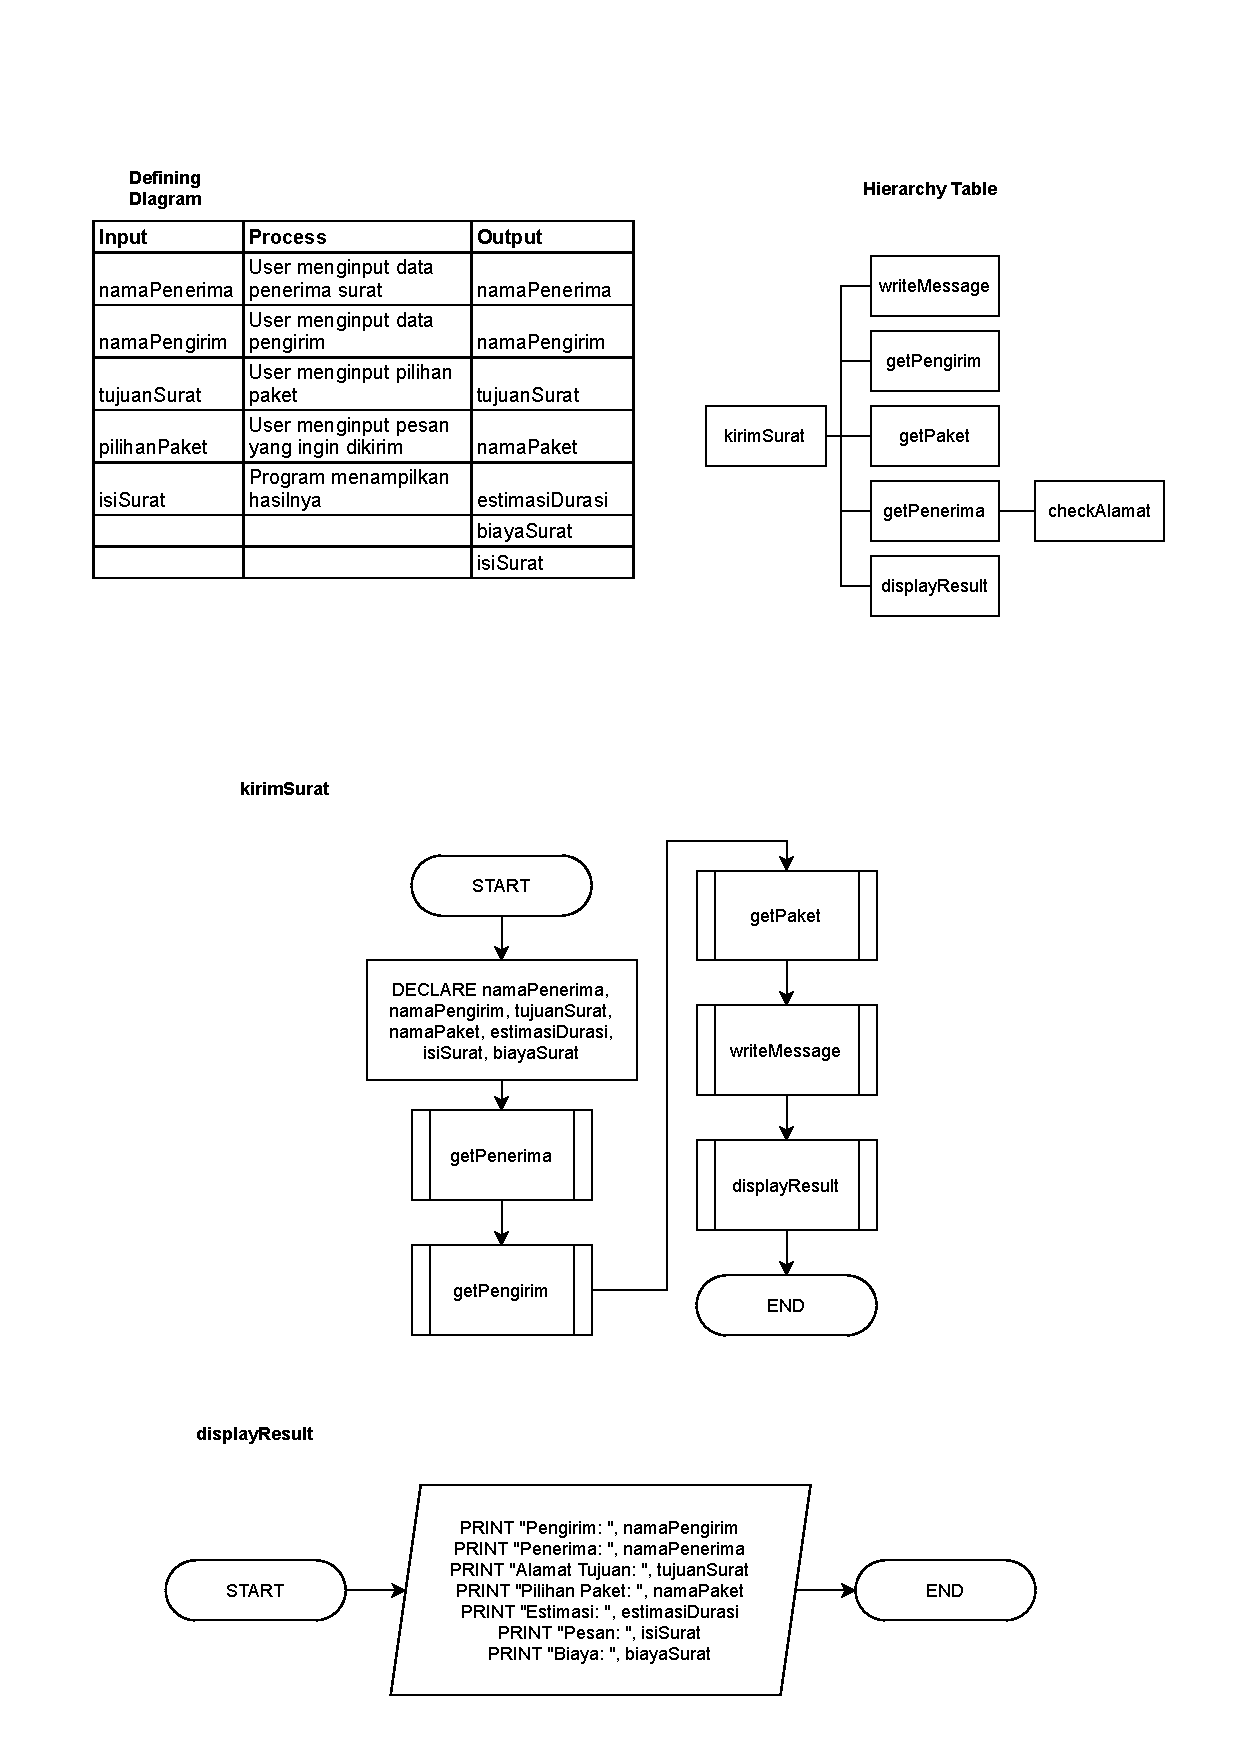
\includegraphics[clip, scale=0.9, trim={1cm 1cm 1cm 3cm}]{pdf/Problem4-1.pdf}
	\end{center}
	\pagebreak
	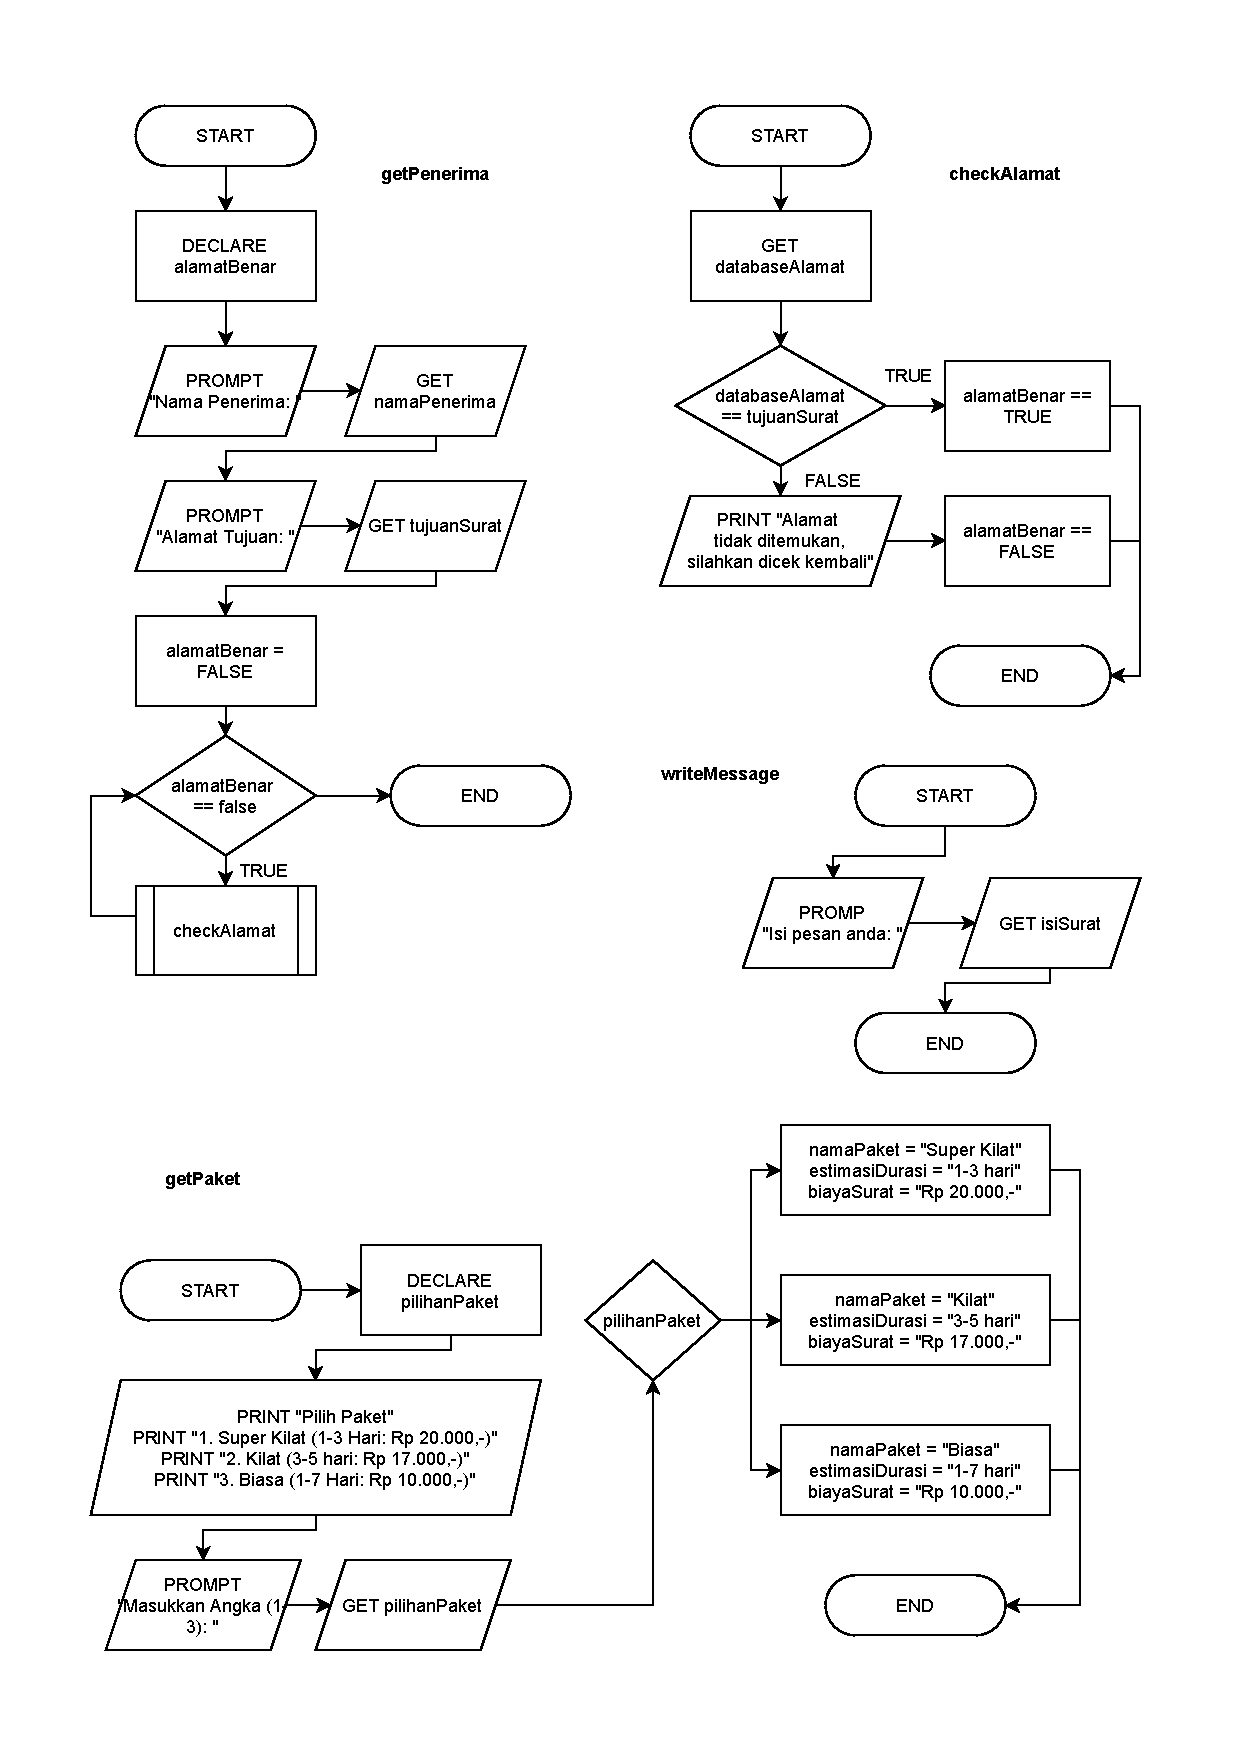
\includegraphics[clip, scale=0.9, trim={1cm 1cm 1cm 1cm}]{pdf/Problem4-2.pdf}
	\subsubsection*{Pseudocode}
	\begin{lstlisting}
kirimSurat
START
1	DECLARE namaPenerima, namaPengirim, tujuanSurat,
	namaPaket, estimasiDurasi, isiSurat, biayaSurat
2	getPenerima()
3	getPengirim()
4	getPaket()
5	writeMessage()
6	displayResult()
END

getPenerima
START
1	DECLARE alamatBenar
2	PROMPT "Nama Penerima: "
	GET namaPenerima
	PROMPT "Alamat Tujuan: "
	GET tujuanSurat
3	alamatBenar = FALSE
4	WHILE (alamatBenar == FALSE)
		checkAlamat()
	ENDWHILE
END

checkAlamat
START
1	GET databaseAlamat
2	IF (databaseAlamat == tujuanSurat)
		alamatBenar == TRUE
	ELSE
		alamatBenar == FALSE
		PRINT "Alamat tidak ditemukan, silahkan dicek kembali"
	ENDIF
END

getPengirim
START
1	PROMPT "Nama Pengirim: "
	GET namaPengirim
END

getPaket()
START
1	DECLARE pilihanPaket
2	PRINT "Pilih Paket"
	PRINT "1. Super Kilat (1-3 Hari: Rp 20.000,-)"
	PRINT "2. Kilat (3-5 hari: Rp 17.000,-)"
	PRINT "3. Biasa (1-7 Hari: Rp 10.000,-)"
	PROMPT "Masukkan angka (1-3: "
3	GET pilihanPaket
4	CASE OF pilihanPaket:
		1: namaPaket = "Super Kilat"
		   estimasiDurasi = "1-3 hari"
		   biayaSurat = "Rp 20.000,-"
		2: namaPaket = "Kilat"
		   estimasiDurasi = "3-5 hari"
		   biayaSurat = "Rp 17.000,-"
		3: namaPaket = "Biasa"
		   estimasiDurasi = "1-7 hari"
		   biayaSurat = "Rp 10.000,-"
END

writeMessage
START
1	PROMPT "Isi pesan anda: "
	GET isiSurat
END

displayResult
START
1	PRINT "Pengirim: ", namaPengirim
	PRINT "Penerima: ", namaPenerima
	PRINT "Alamat Tujuan: ", tujuanSurat
	PRINT "Pilihan Paket: ", namaPaket
	PRINT "Estimasi: ", estimasiDurasi
	PRINT "Pesan: ", isiSurat
	PRINT "Biaya: ", biayaSurat
END
	\end{lstlisting}

	\subsection*{Desk Checking}
	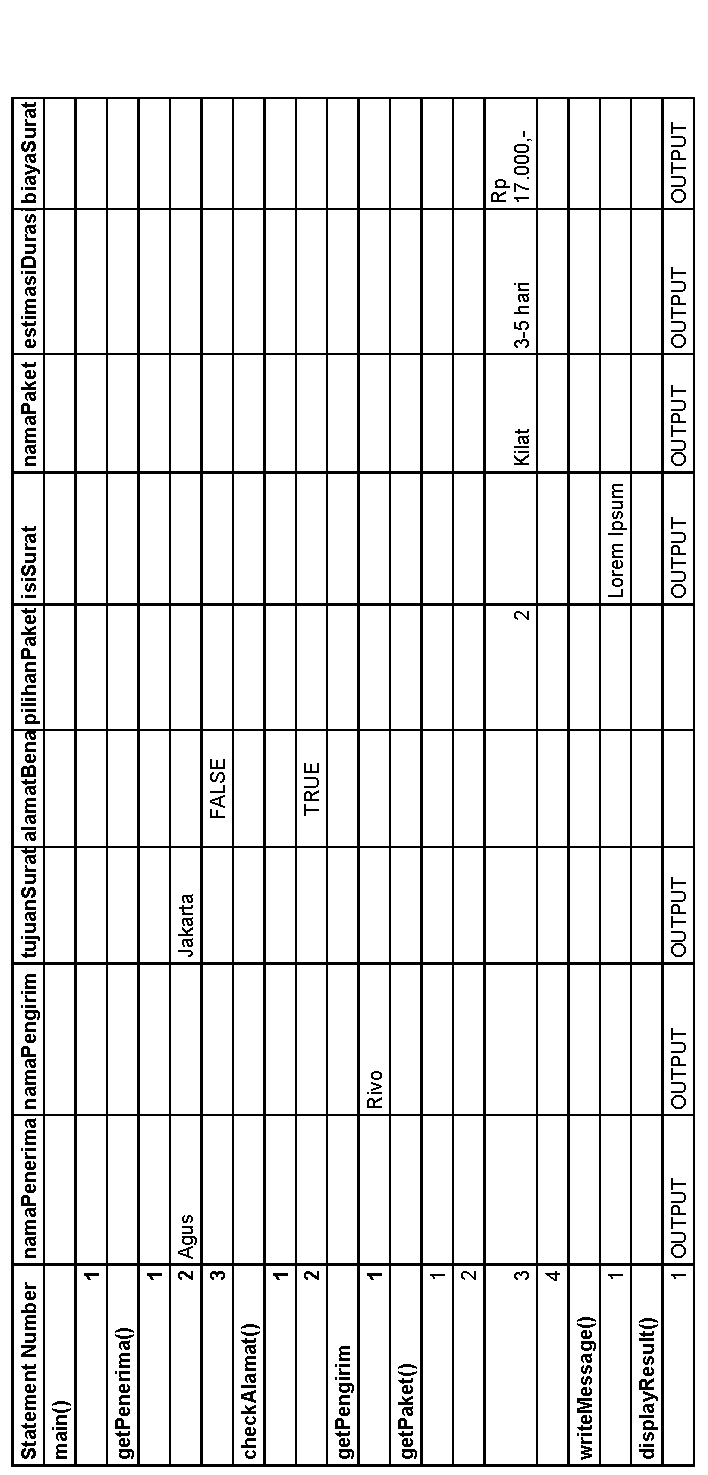
\includegraphics[clip]{pdf/Problem4DC.pdf}
\end{document}
